\section{Process' perspective}
\subsection{Complete description of CI/CD pipeline}
In order to create a seamless integration of new updates in the code with a focus on high confidence of the quality of the code, we have created a CI/CD pipeline. All code which is passed on to the deployed production environment will have to go through two stages. The first pipeline triggers on the creation of a GitHub pull-request, and the second triggers when a pull-request is approved and a merge happens with the main branch. 
\begin{figure}[H]
    \centering
    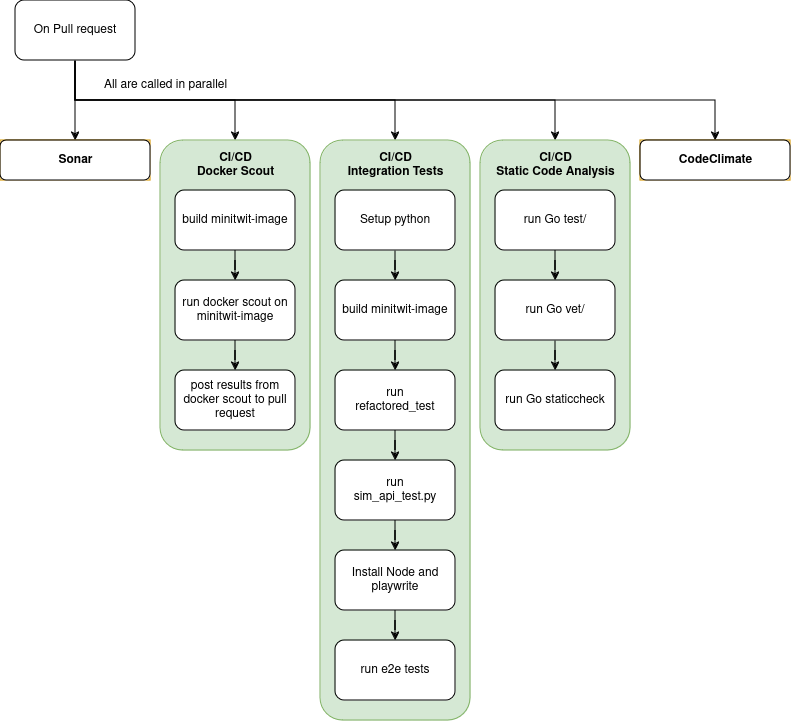
\includegraphics[scale=.5]{diagrams/PullRequest_CICD.png}
    \caption{Diagram showing the CI/CD actions run when a pull request is created.}
    \label{fig:pull request ci/cd}
\end{figure}
When a pull-request is created five actions are run, which can be seen in figure \ref{fig:pull request ci/cd}. The actions run are \texttt{SonarCloud}, and \texttt{CodeClimate} which scan the code and evaluate the linting of the code as well as code practices. Secondly, we also run docker scout, self written integration tests, and a static code analysis tool, which have their execution defined through \texttt{.yml} files within the repository. All the actions mentioned priorly are run in parallel and show each their own report on the pull request, see figure  
\begin{figure}[H]
    \centering
    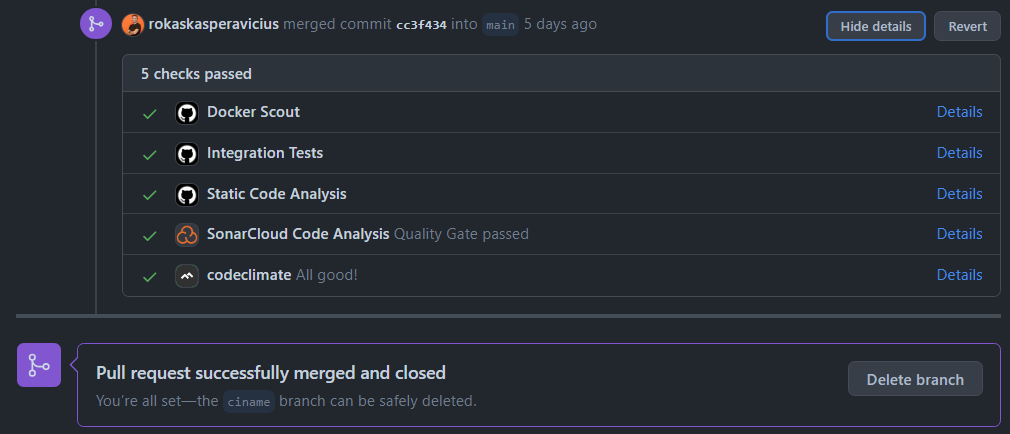
\includegraphics[width=0.8\linewidth]{img/pullRequestReportings.png}
    \caption{Screenshot showing each action on a pull request.}
    \label{fig:PR reportings}
\end{figure}

Once a pull request has been reviewed and is approved for merge, the second pipeline activates. The purpose of this pipeline is to ensure that once changes are added to the main branch of the git, they are synchronized with our production environment. This pipeline consists of two different actions, where the first action synchronizes the contents of the main branch with the digital ocean droplet. 
\\
\\
The second action is dependant on the first actions completion, and will only execute once the first action is finished. The second action creates an automatically generated release on the GitHub page, incrementing the minor version number by one and publishing all the commits in a collected report. 
\begin{figure}[H]
    \centering
    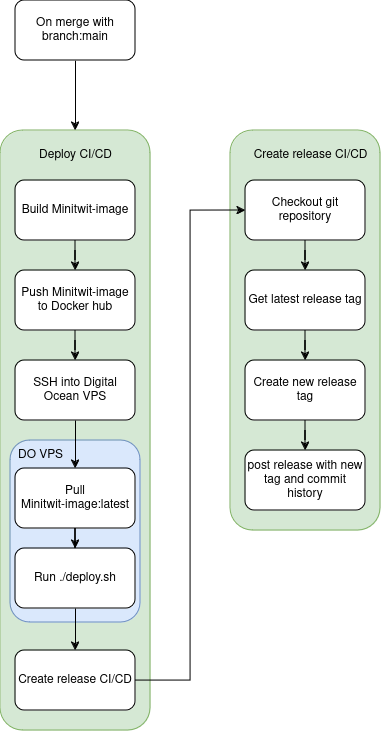
\includegraphics[scale=.5]{diagrams/MergeMain_CICD.png}
    \caption{Diagram showing the CI/CD actions run when git detects a merge into main.}
    \label{fig:merge with main ci/cd}
\end{figure}


\subsection{Monitoring - Grafana and Prometheus}

Prometheus and Grafana are powerful tools to measure and visualise our system metrics. Prometheus is gathering the system metrics, whereas Grafana provides visualising capabilities to gain valuable knowledge about the performance and health of our system  \cite{slides}.
\\
\\
The tools are configured in our \texttt{docker-compose.prod.yml} file as separate Docker containers on our manager node. Docker volumes are used to persist data and configurations between the host system and containers, allowing us to decouple the data storage from the container lifecycles. The Prometheus container uses a prom/prometheus image and a custom Prometheus configuration file \texttt{prometheus.yml}, that scrapes the /metrics endpoint of our API every 10 seconds. The volume \texttt{prom\_data} persists Prometheus data, such as metrics and other operational data, across container lifecycles.
\\
\\
The Grafana container uses the latest grafana/grafana image and a custom datasource configuration file \texttt{datasource.yml}, which specifies the connection between Grafana and the prometheus host on port 9090 in the Docker Swarm network. The volume \texttt{grafana\_data} stores persistent data such as dashboards and other operational data that is essential for Grafana.
\\
\\
We have instrumented different prometheus metrics counters in our backend, which track the application performance by the number of user registrations, messages, follows and unfollows. In addition to this, we are tracking the total count of responses for different handlers, status codes and methods, which allow us to pinpoint where errors occur and take corrective measures. Finally, we have set up an alert in Grafana, which alerts our communication channel in the event of downtime on a worker node. The dashboards can be viewed below. 

 \begin{figure}[H]
    \centering
    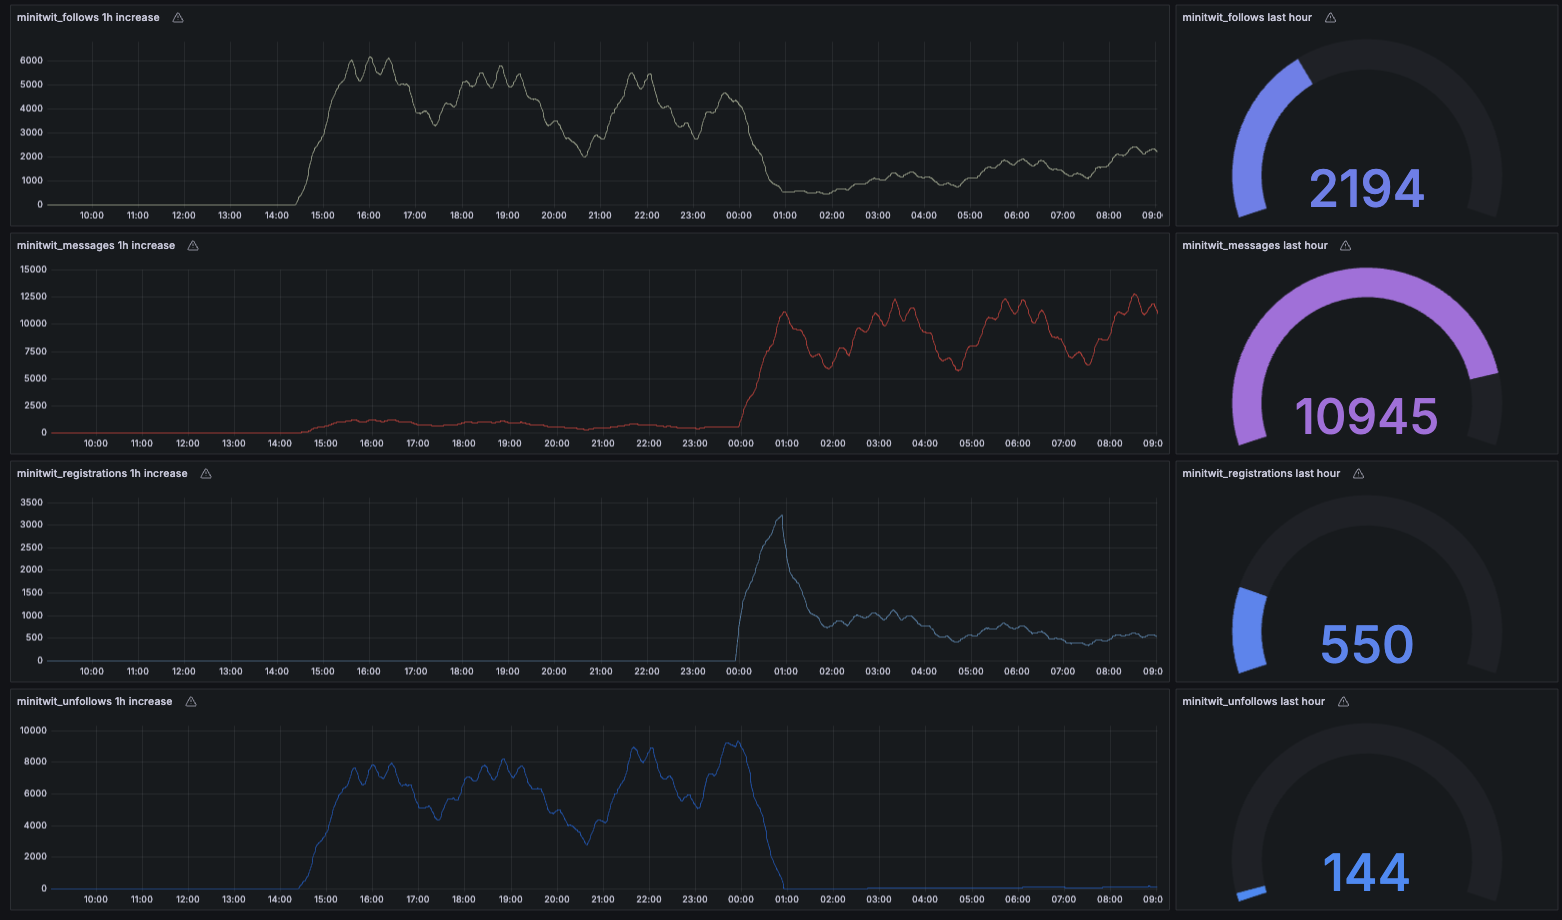
\includegraphics[scale=.3]{img/increases.png}
    \caption{Grafana dashboards showing the number of registrations, messages, follows and unfollows in the last hour.}
\end{figure}

\begin{figure}[H]
    \centering
    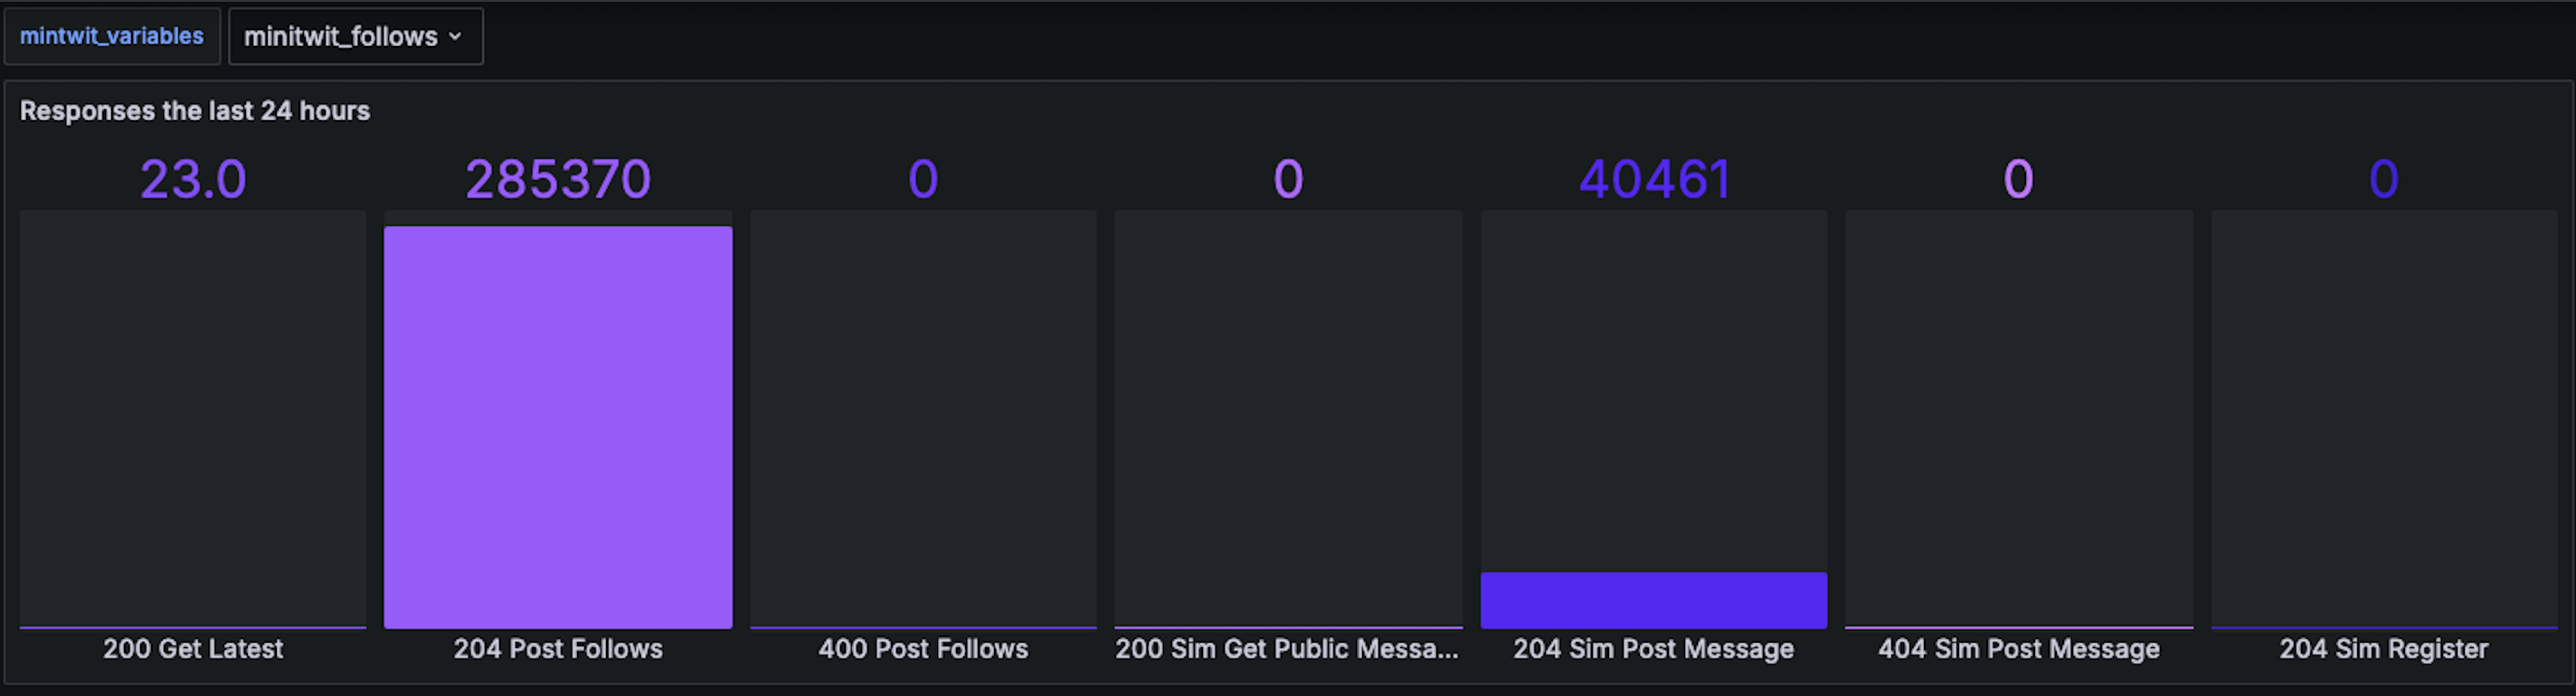
\includegraphics[scale=.33]{img/responses.png}
    \caption{Grafana dashboard showing the total count of responses for different handlers, status codes and methods in the last 24 hours.}
\end{figure}

\newpage
\subsection{Logging}
% plugins on the workers  (called: ) which send both stderr and stdout to the manager node. The manager node contains the graphana instance which displays the logs. 
% https://grafana.com/docs/loki/latest/send-data/docker-driver/
In order to allow us to understand an error which might have occurred in the system, we make use of logging. In order to log the status of the system, we use a docker container of Loki, running on the manager. Additionally, we have installed a Loki plugin on each worker in the system, which listens to the \texttt{stdErr} and the \texttt{stdOut} of the workers. Anything which is written to either, will be passed from the worker by the plug-in, to the Loki image on the manager. In order to allow us to read the logs we make use of the Grafana image, which connects to the Loki image, and displays the logs. See figure \ref{fig:loki in grafana}.

\begin{figure}[H]
    \centering
    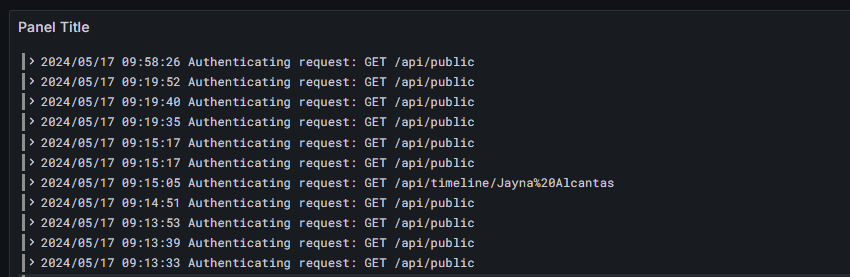
\includegraphics[width=.8\linewidth]{img/Logs.png}
    \caption{Screenshot of logs displayed in Grafana.}
    \label{fig:loki in grafana}
\end{figure}

\subsection{Security}
To ensure the application was secure we have implemented multiple practices. 
Firstly, the project was initially analyzed with two tools which returned a report on possible vulnerabilities; \texttt{Nmap} and \texttt{skipfish}. The first tool, \texttt{Nmap}, tried pinging every port within our application to find which ports were in use. This could help us spot any potential entry-points into our system, which might have been opened on accident. The results of the \texttt{Nmap} scan can be seen in listing \ref{nmap_results}.
\begin{lstlisting}[frame = trBL, label=nmap_results, caption={Listing of the report returned by Nmap}]
Starting Nmap 7.94SVN ( https://nmap.org ) at 2024-04-19 11:33 UTC
Nmap scan report for 138.68.126.8
Host is up (0.019s latency).
Not shown: 997 closed tcp ports (reset)
PORT     STATE SERVICE VERSION
22/tcp   open  ssh     OpenSSH 8.9p1 Ubuntu 3ubuntu0.6 
80/tcp   open  http
5000/tcp open  upnp?
\end{lstlisting}
These results show us that the only publicly exposed ports are port 22, 80, and 5000. All these ports are intended to be open. 
\\
\\
The second tool, skipfish, created a scan which looked through the code, in-search of deprecated libraries, unsafe file types or other vulnerabilities. The results from skipfish can be seen in the GitHub repository\footnote{Skipfish results found here: 
\href{https://github.com/DevOps-Ben11/minitwit/tree/main/skipfish/}{github.com/DevOps-Ben11/minitwit/tree/main/skipfish}}.
\\
\\
Finally to ensure that the security of the project is upheld through development, we integrated security analysis tools into the CI/CD pipeline. Here, SonarCloud has security oriented quality gates which need to pass in order for the pull request to be approved. Additionally, docker scout was implemented. The docker scout action will build the current version of the system and scan the docker image for any vulnerabilities. The results will be compiled into a report and shown on the pull-request. See figure \ref{fig:docker scout report}.
\begin{figure}[H]
    \centering
    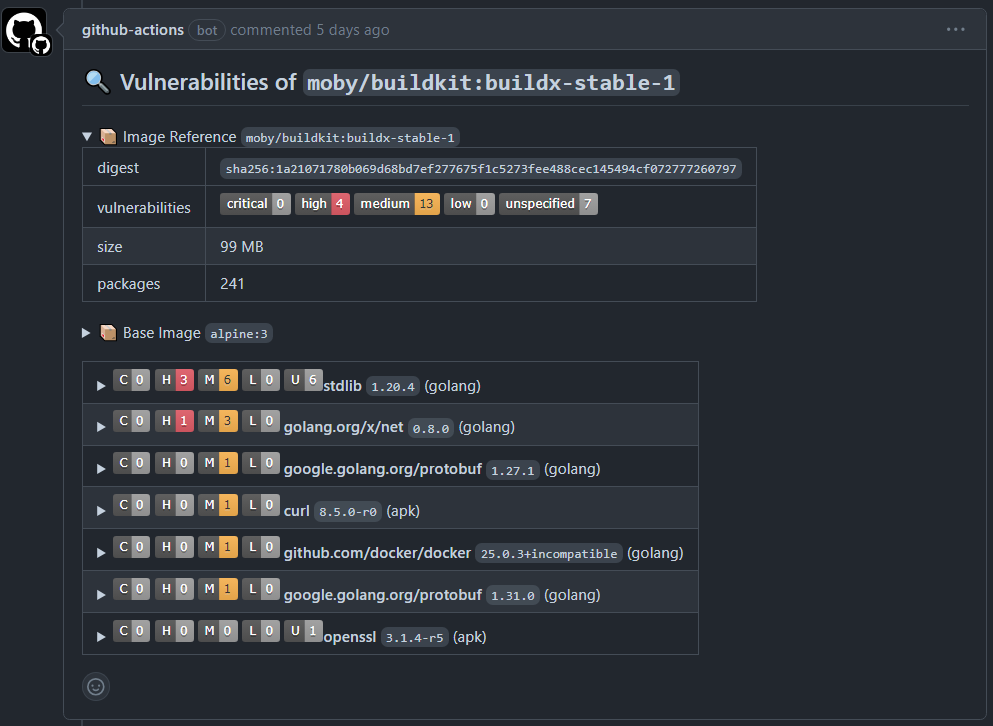
\includegraphics[width=.8\linewidth]{img/dockerScoutReport.png}
    \caption{Screenshot showing the reports of docker scout and which potential vulnerabilities there might be within our system.}
    \label{fig:docker scout report}
\end{figure}
In figure \ref{fig:docker scout report} the report of docker scout is shown. Here, the reviewer of the pull-request can see which potential security vulnerabilities there might be within the update to the system. In this specific case we see that there are 3 high, 6 medium, and 6 unspecified vulnerabilities in the standard library of Go-Lang, the language the backend is written in.

\subsection{Applied strategy for scaling}
We have applied Docker Swarm to support advanced scaling by distributing the load across multiple nodes. The Docker Swarm structure of our system can be viewed in \textit{Figure} \ref{fig:overall_system}. The swarm is a cluster of hosts in a distributed system. The swarm has a manager node, that acts as a load balancer by routing the traffic to the worker nodes. The manager node assigns the worker nodes tasks, such as running containers, serving traffic and handling application logic. When the system is scaled up or down, the manager node will automatically adapt the tasks to the desired state \cite{swarm}. 
\\
\\
The Docker service \texttt{minitwit-image} is running in a global mode constrained to the worker nodes, such that exactly one replica of the service is deployed to each worker node. The restart-policy is set to \texttt{any}, such that the service restarts in the event of any problem. The update strategy is set to the blue-green strategy, such that new tasks are initiated before old tasks are stopped to secure high availability.  
\\
\\
The swarm ensures a highly available system by applying horizontal scaling. This enables us to easily replicate services and add more worker nodes to the cluster according to our needs. The load balancer ensures a highly available system by distributing the traffic evenly across the worker nodes. To create an even more redundant system, we could remove the single point of failure by introducing more manager nodes. In the event of failure on the leading manager node, another manager would be appointed and take over the tasks \cite{slides9}. 
\\
\\
We have applied infrastructure as code to support vertical scaling of our system with Terraform. The Terraform folder in our repository contains the configuration file \texttt{main.tf}, the environmental variables file \texttt{terraform.tfvars}, and the state file \texttt{terraform.tfstate}. Terraform keeps track of the infrastructure state in the \texttt{terraform.tfstate} file and plans to update the state with the desired state in the \texttt{main.tf} file. 
Terraform automatically loads the environmental variables from the \texttt{terraform.tfvars} file.
\\
\\
The configuration file \texttt{main.tf} creates three digital ocean droplets named \textit{manager}, \textit{worker-1} and \textit{worker-2} defined as resources with the connection set to ssh. In the configuration of the manager resource, we are provisioning files from the host to the droplet, running remote-exec commands on the droplet for setting permissions, storing environmental variables, initialising the swarm, storing the swarm\_token, and running the visualiser. In the configuration of each worker resource, we are running remote-exec commands to copy the swarm\_token from the manager to the worker to join the swarm. In all the resources, we need to install the Docker plugin for Loki and set the Firewall to allow traffic from the swarm. 
\\
\\
Terraform supports vertical scaling, which only requires us to change the configurations of the droplets in the \texttt{main.tf} file and run the CLI commands \textit{terraform init}, \textit{terraform plan} and \textit{terraform apply}, which reloads the droplet with the desired configurations. Terraform allows us to take down our system and relaunch it for the exam with minimal effort \cite{terraform}. 



